\section{Langkah-Langkah Percobaan}
\subsection{Routing Statis IPv6}
\begin{enumerate}
    \item Kabel Lan dihubungkan ke laptop ke router,dan router ke router.
    \item Login menggunakan MAC address,lalu router direset terlebih dahulu menggunakan Winbox.
    \begin{figure}[H]
        \centering
        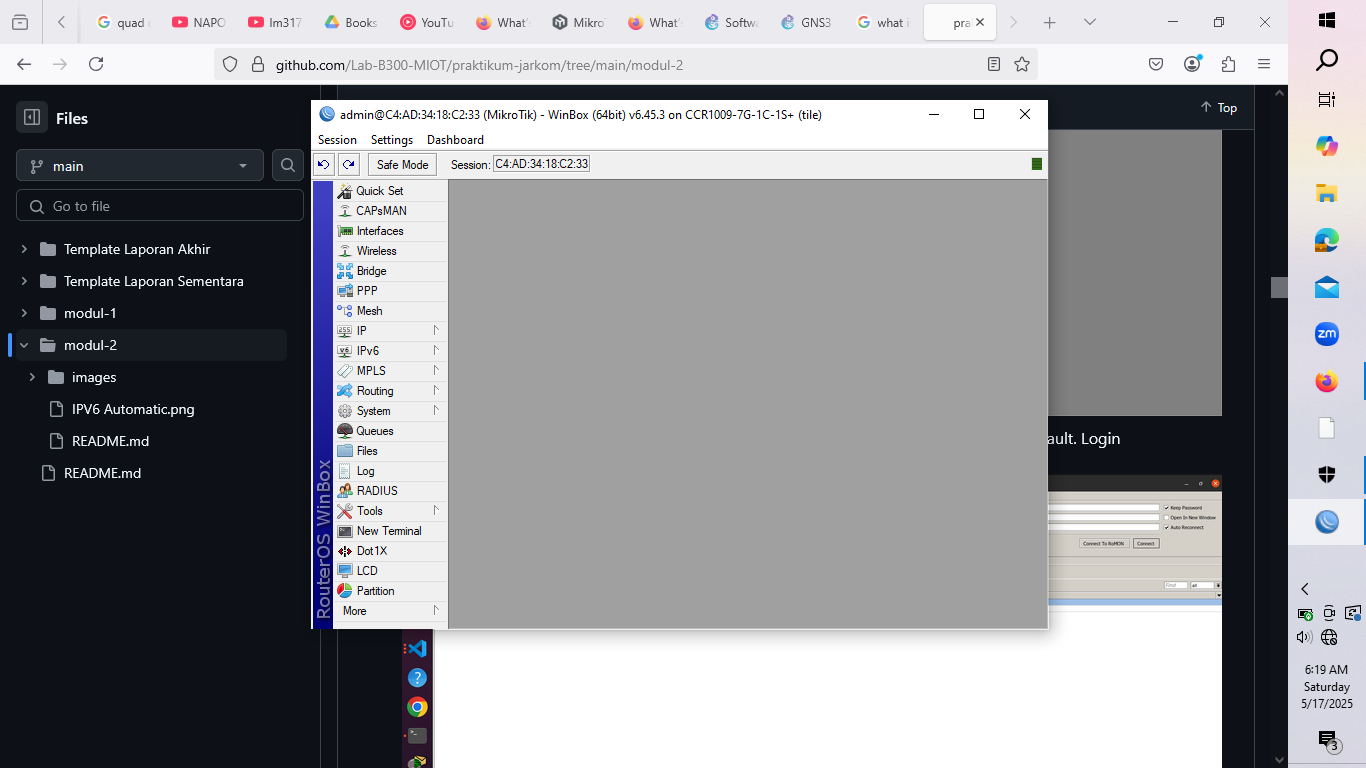
\includegraphics[width=0.5\linewidth]{gambar1.png}
        \caption{Mereset Router pada Winbox}
        \label{fig:gambar1}
    \end{figure}
    \item IPv6 di aktifkan pada menu IPv6, dan masukkan IPv6 address pada menu IPv6 address Untuk setiap
    laptop.
    \begin{figure}[H]
        \centering
        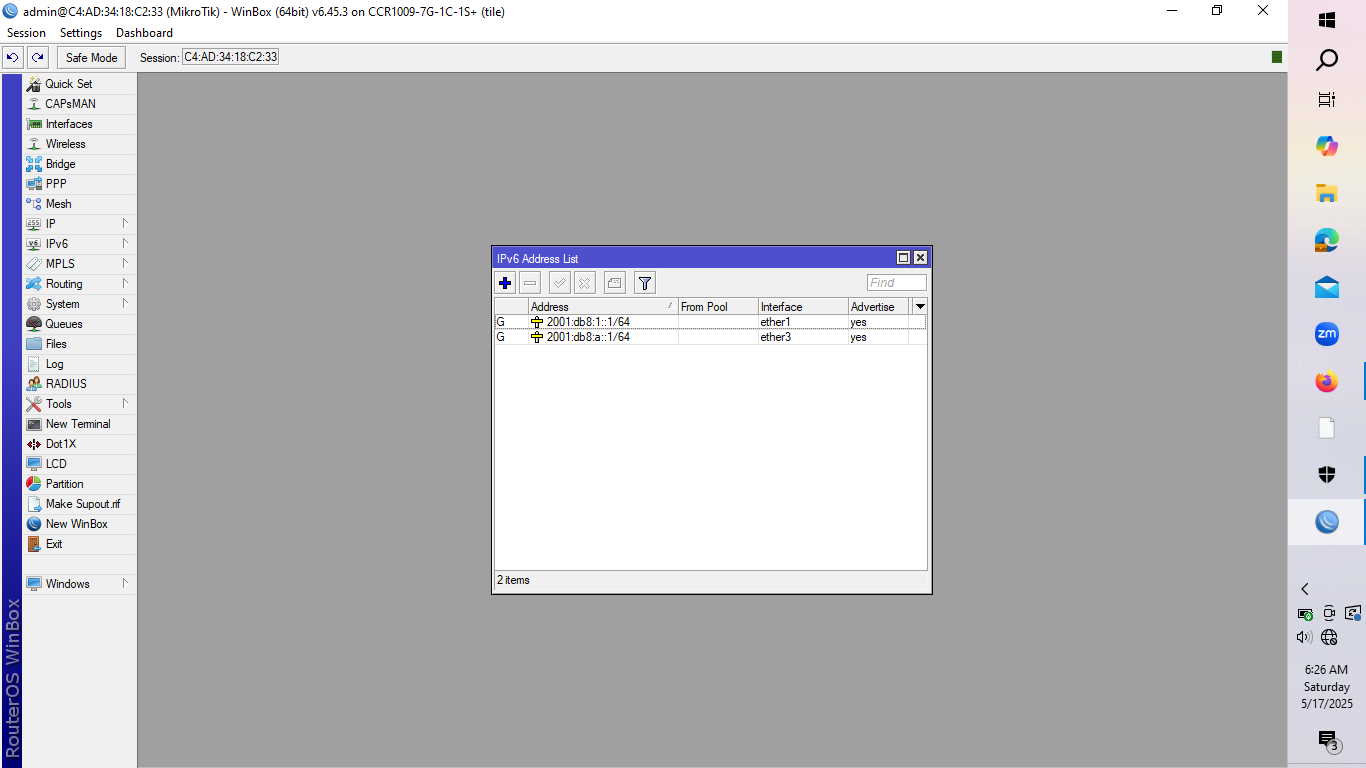
\includegraphics[width=0.5\linewidth]{gambar2.png}
        \caption{Mengaktifkan IPv6 pada Router}
        \label{fig:gambar2}
    \end{figure}
    \item Tambahkan rute pada menu IPv6 route.
    \begin{figure}[H]
        \centering
        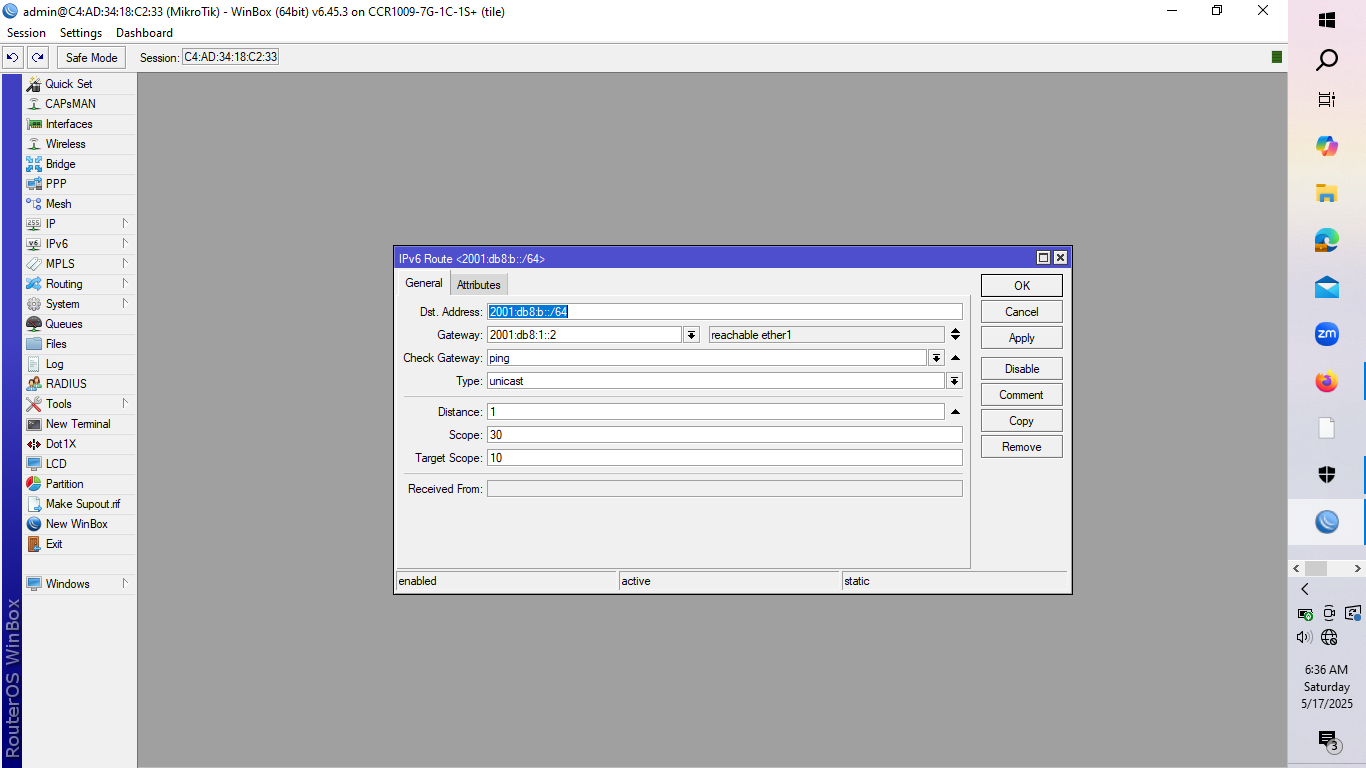
\includegraphics[width=0.5\linewidth]{gambar3.png}
        \caption{Menambahkan Rute IPv6 pada Router}
        \label{fig:gambar3}
    \end{figure}
    \item Konfigurasiknan IPv6 pada laptop menggunakan IPv6 address yang telah ditentukan melalui menu
    setting pada laptop.
    \begin{figure}[H]
        \centering
        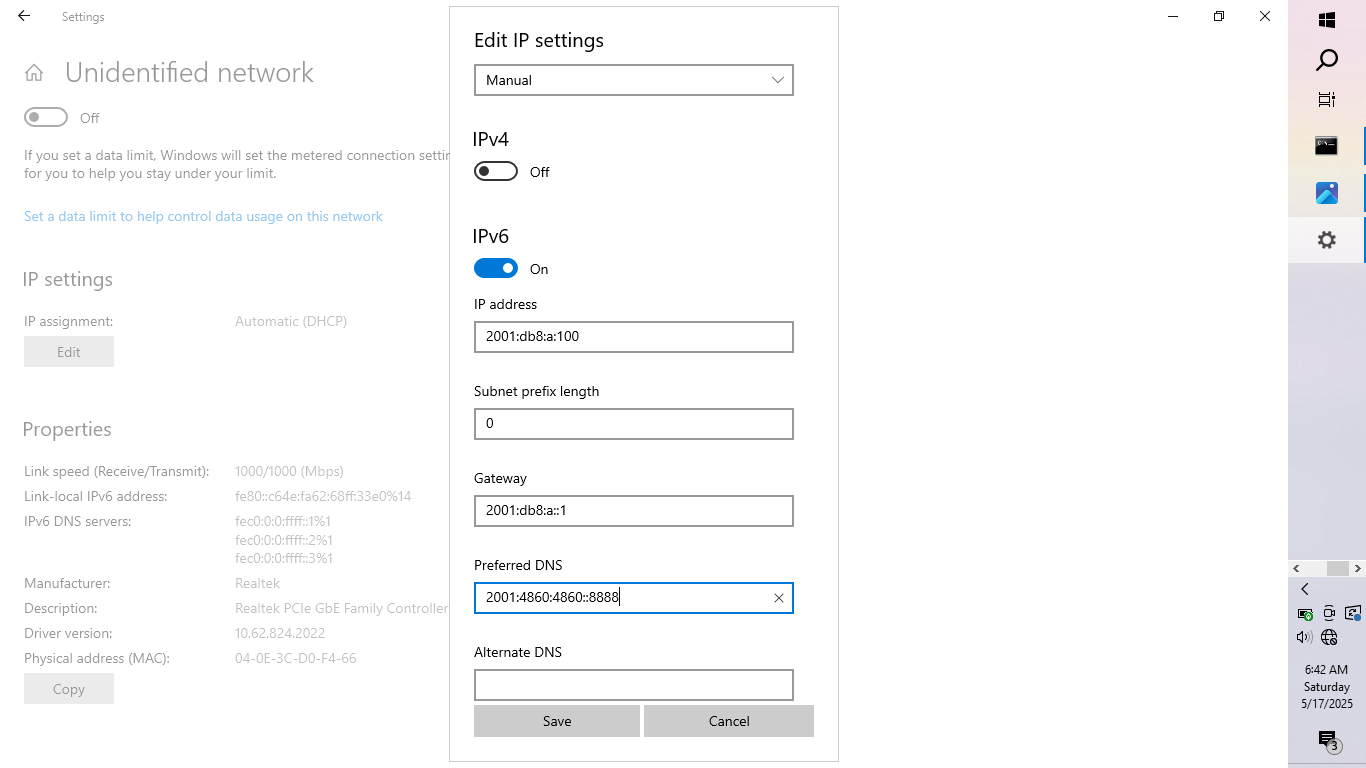
\includegraphics[width=0.5\linewidth]{gambar4.png}
        \caption{Mengkonfigurasi IPv6 pada Laptop}
        \label{fig:gambar4}
    \end{figure}
    \item Setelah semua konfigurasi selesai, lakukan ping dari laptop ke router dan ke laptop lain untuk
    memastikan koneksi antar laptop dan router sudah terhubung.
    \begin{figure}[H]
        \centering
        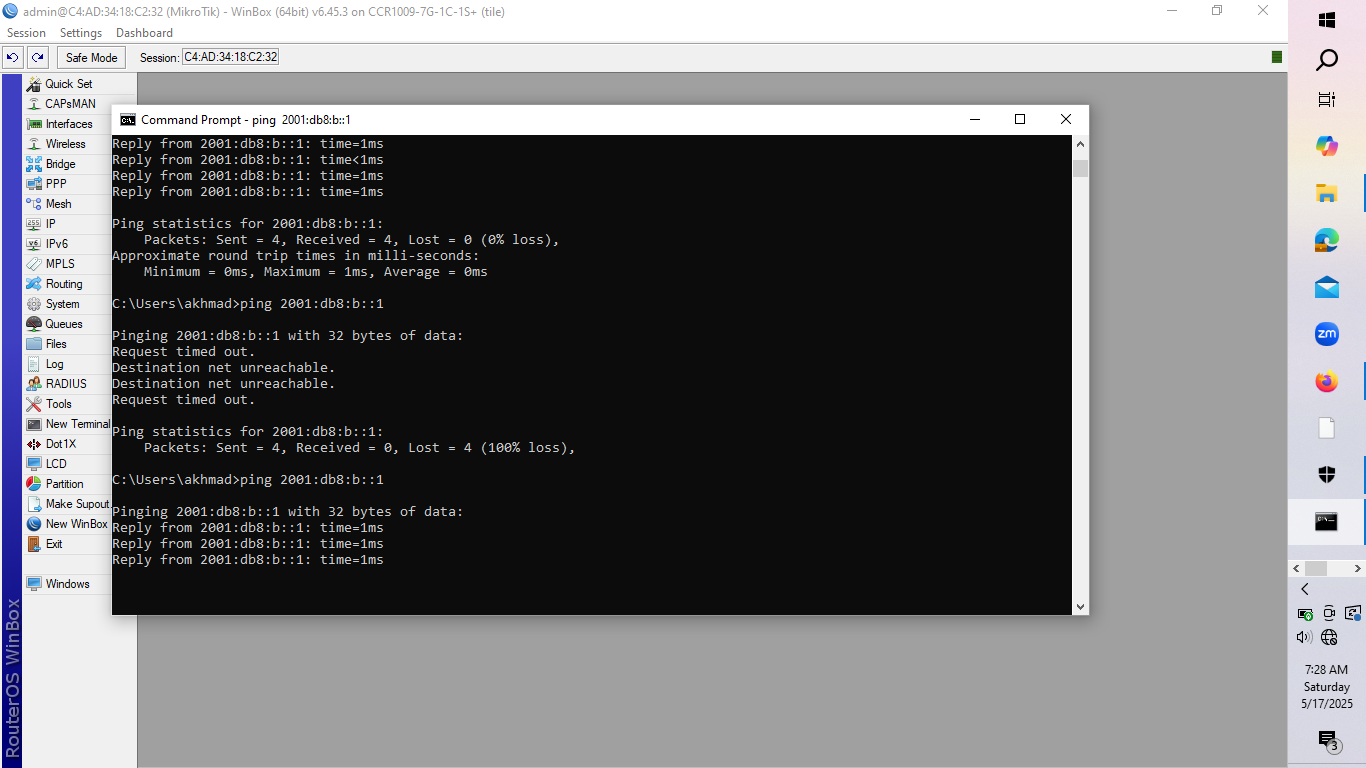
\includegraphics[width=0.5\linewidth]{ping.png}
        \caption{Melakukan Ping dari Laptop ke Router}
        \label{fig:gambar5}
    \end{figure}
\end{enumerate}


\subsection{Routing Dinamis IPv6}
\begin{enumerate}
    \item Login menggunakan MAC address,lalu router direset terlebih dahulu menggunakan Winbox.
    \begin{figure}[H]
        \centering
        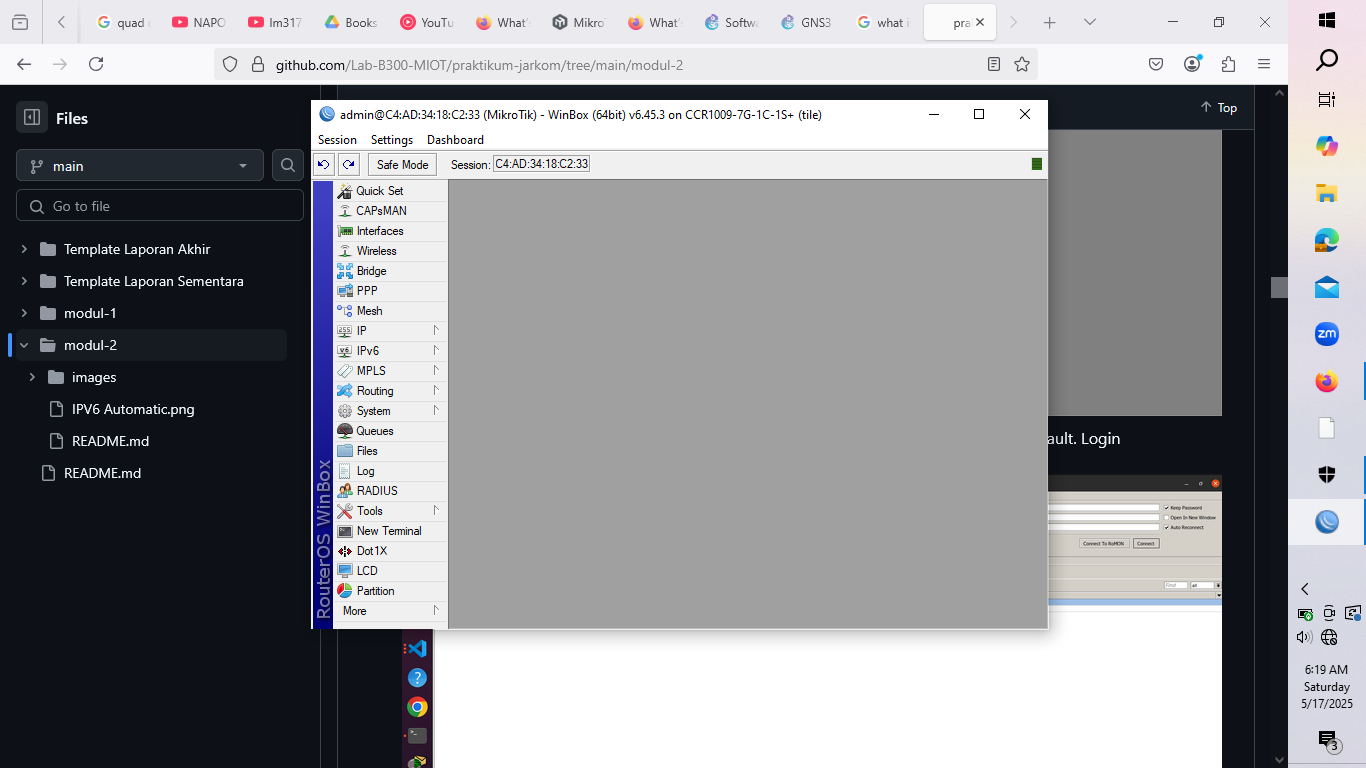
\includegraphics[width=0.5\linewidth]{gambar1.png}
        \caption{Mereset Router pada Winbox}
        \label{fig:gambar1}
    \end{figure}
    \item IPv6 di aktifkan pada menu IPv6, dan masukkan IPv6 address pada menu IPv6 address Untuk setiap
    laptop.
    \begin{figure}[H]
        \centering
        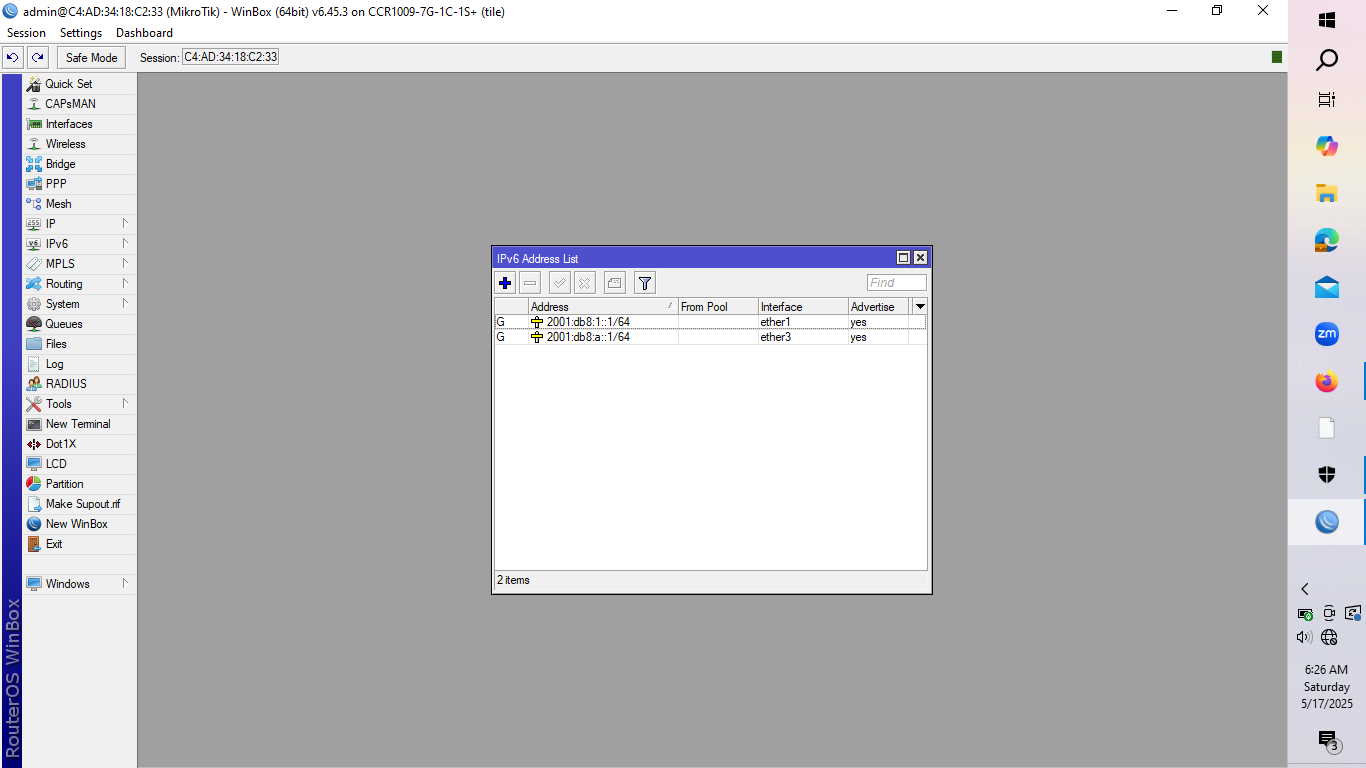
\includegraphics[width=0.5\linewidth]{gambar2.png}
        \caption{Mengaktifkan IPv6 pada Router}
        \label{fig:gambar2}
    \end{figure}
    \item Buat instance OSPF pada menu OSPF instance dengan nama ospf-instance.
    \begin{figure}[H]
        \centering
        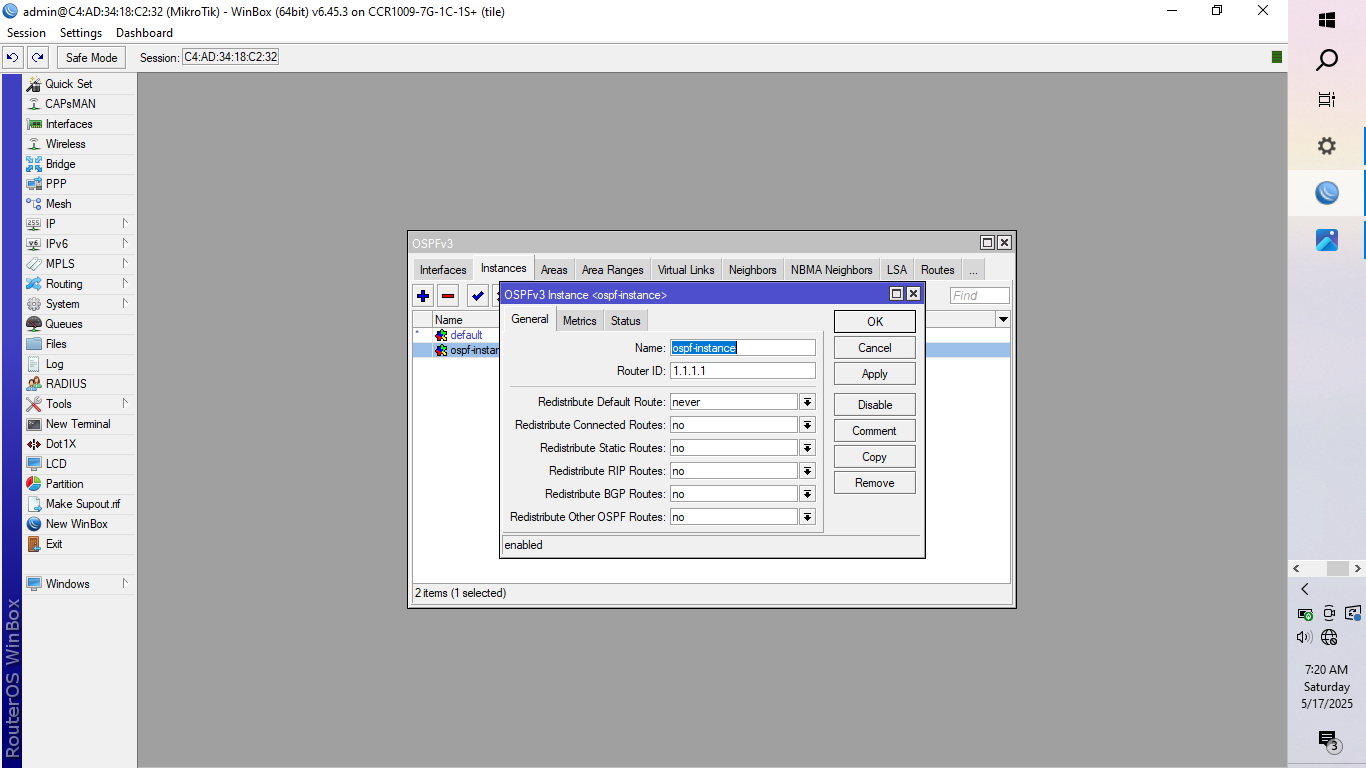
\includegraphics[width=0.5\linewidth]{gambar5.png}
        \caption{Membuat Instance OSPF pada Router}
        \label{fig:gambar6}
    \end{figure}    
    \item Lalu tambahkan area OSPF pada menu OSPF area dengan nama area1.
    \begin{figure}[H]
        \centering
        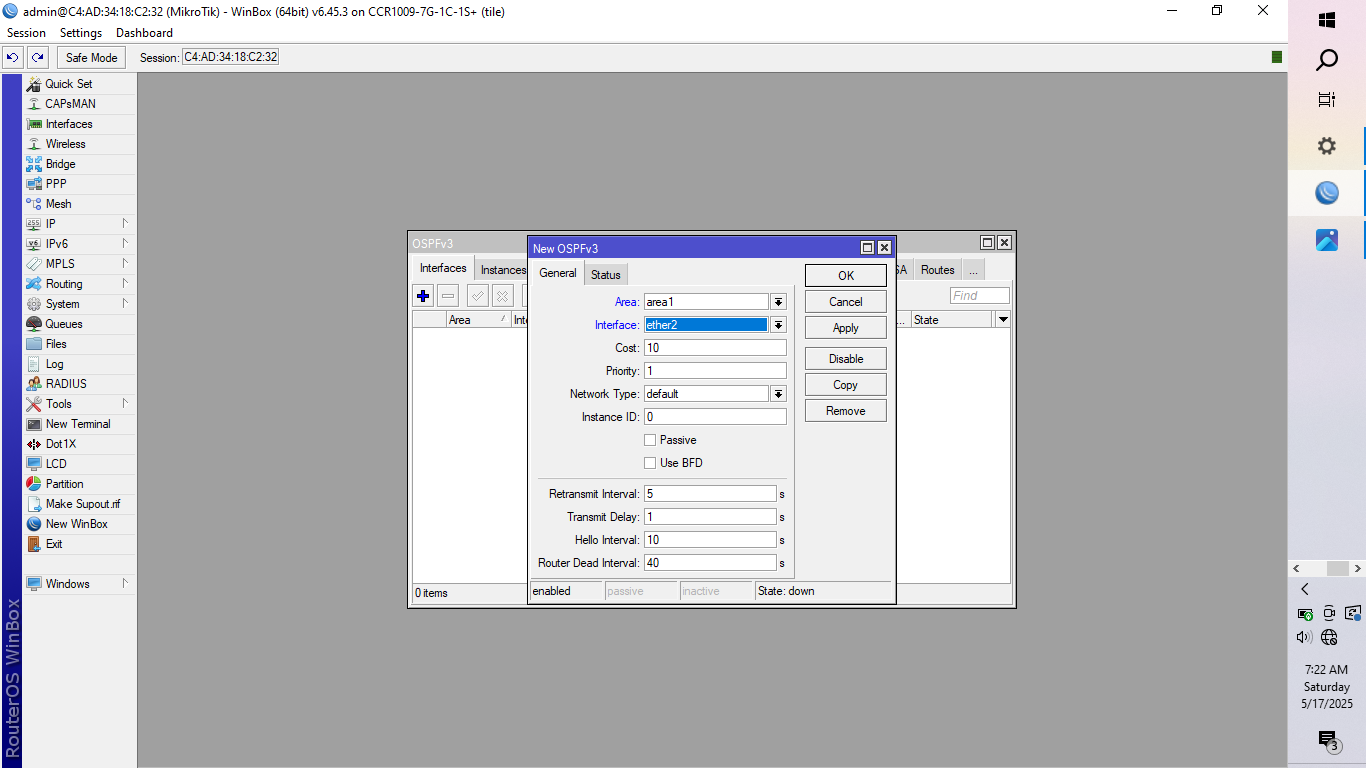
\includegraphics[width=0.5\linewidth]{gambar6.png}
        \caption{Menambahkan Area OSPF pada Router}
        \label{fig:gambar7}
    \end{figure}
    \item Tambahkan interface pada menu OSPF untuk setiap interface yang ada pada router.
    \begin{figure}[H]
        \centering
        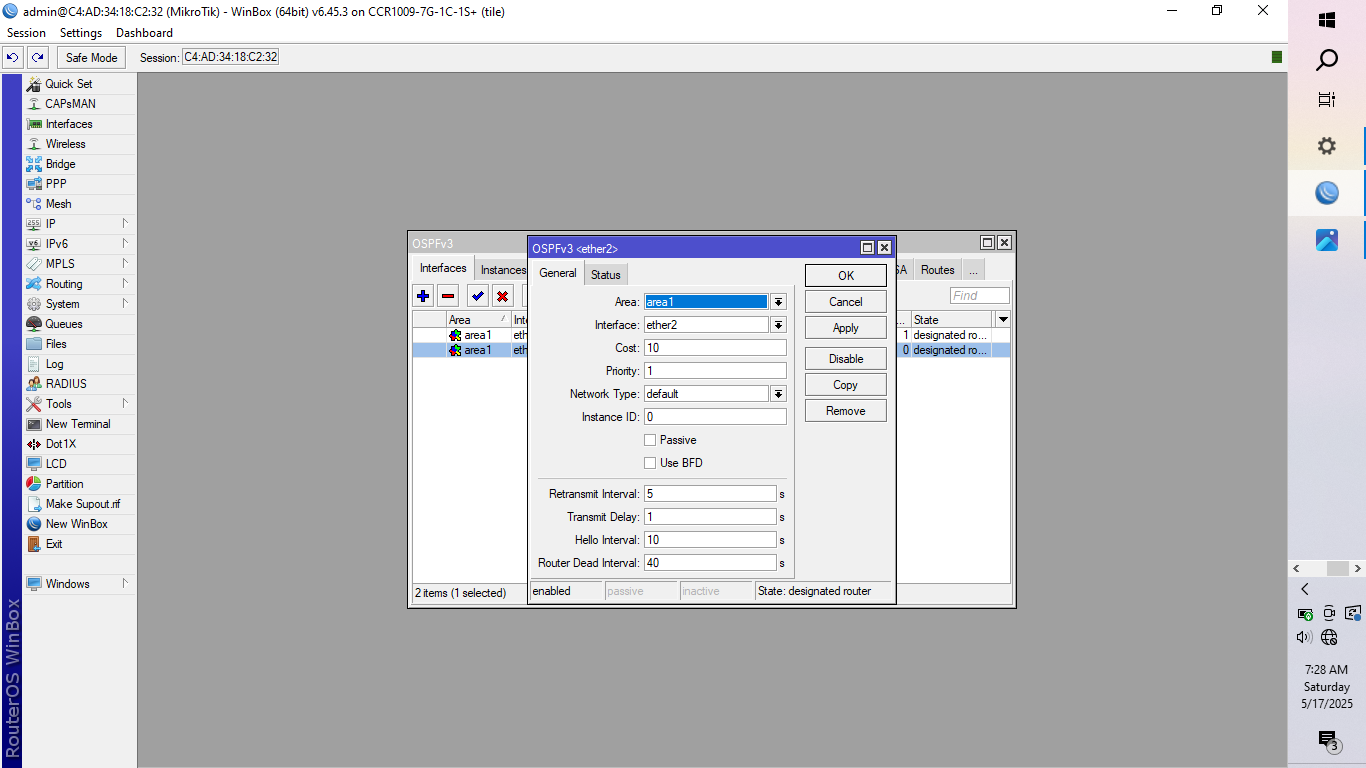
\includegraphics[width=0.5\linewidth]{gambar7.png}
        \caption{Menambahkan Interface OSPF pada Router}
        \label{fig:gambar8}
    \end{figure}
        \item Konfigurasiknan IPv6 pada laptop menggunakan IPv6 address yang telah ditentukan melalui menu
    setting pada laptop.
    \begin{figure}[H]
        \centering
        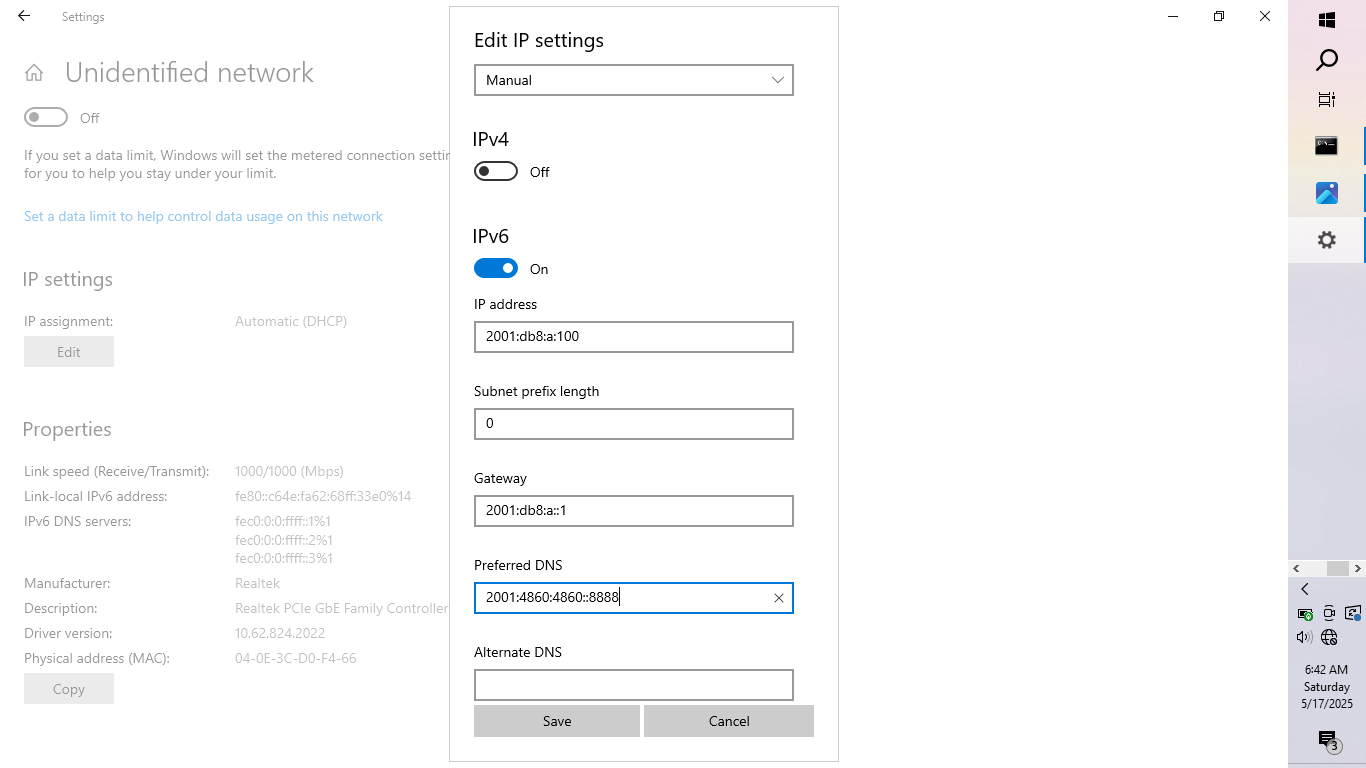
\includegraphics[width=0.5\linewidth]{gambar4.png}
        \caption{Mengkonfigurasi IPv6 pada Laptop}
        \label{fig:gambar4}
    \end{figure}
    \item Setelah semua konfigurasi selesai, lakukan ping dari laptop ke router dan ke laptop lain untuk
    memastikan koneksi antar laptop dan router sudah terhubung.
    \begin{figure}[H]
        \centering
        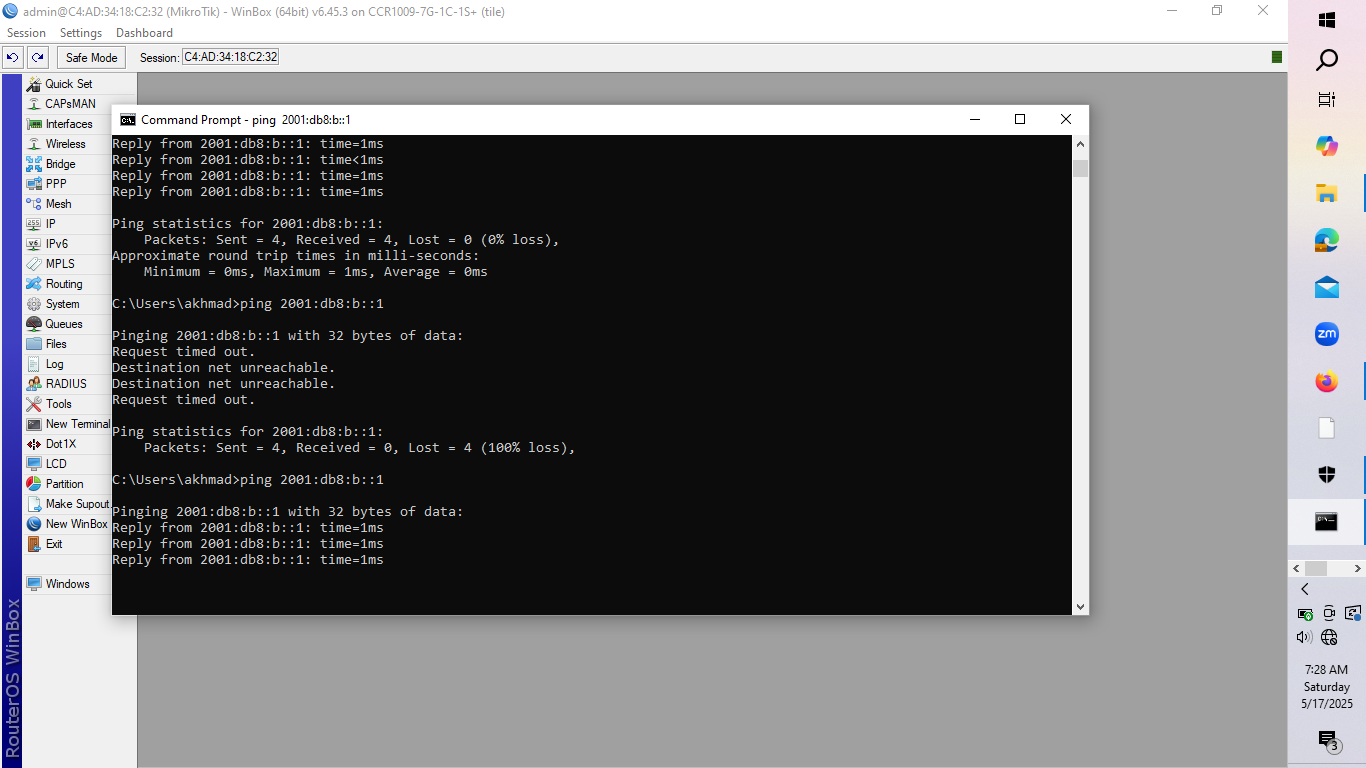
\includegraphics[width=0.5\linewidth]{ping.png}
        \caption{Melakukan Ping dari Laptop ke Router}
        \label{fig:gambar5}
    \end{figure}
    
\end{enumerate}

\section{Analisis Hasil Percobaan}
Pada hasil percobaan routing statis IPv6, dapat dilihat bahwa semua laptop dapat saling terhubung satu sama lain
dan dapat melakukan ping ke router. Hal ini menunjukkan bahwa routing statis IPv6 berhasil dilakukan dengan baik.
Pada hasil percobaan routing dinamis IPv6, dapat dilihat bahwa semua laptop dapat saling terhubung satu sama lain
dan dapat melakukan ping ke router. Hal ini menunjukkan bahwa routing dinamis IPv6 juga berhasil dilakukan dengan baik.
Namun, routing dinamis IPv6 lebih efisien dibandingkan dengan routing statis IPv6 karena routing dinamis
IPv6 dapat menyesuaikan diri dengan perubahan topologi jaringan secara otomatis, sedangkan routing statis IPv6
harus dikonfigurasi secara manual setiap kali terjadi perubahan topologi jaringan. Pada routing dinamis IPv6 digunakan
OSPF sebagai protokol routing yang dapat menyesuaikan diri dengan perubahan topologi jaringan secara otomatis.OSPF
merupakan protokol routing yang menggunakan algoritma Dijkstra untuk menentukan jalur terpendek ke tujuan.
Dengan menggunakan OSPF, router dapat saling bertukar informasi routing dan membangun tabel routing secara otomatis.
Dengan demikian, routing dinamis IPv6 lebih efisien dan lebih mudah dikelola dibandingkan dengan routing statis IPv6.

\section{Hasil Tugas Modul}

\begin{enumerate}
    \item  
    \begin{figure}[H]
        \centering
        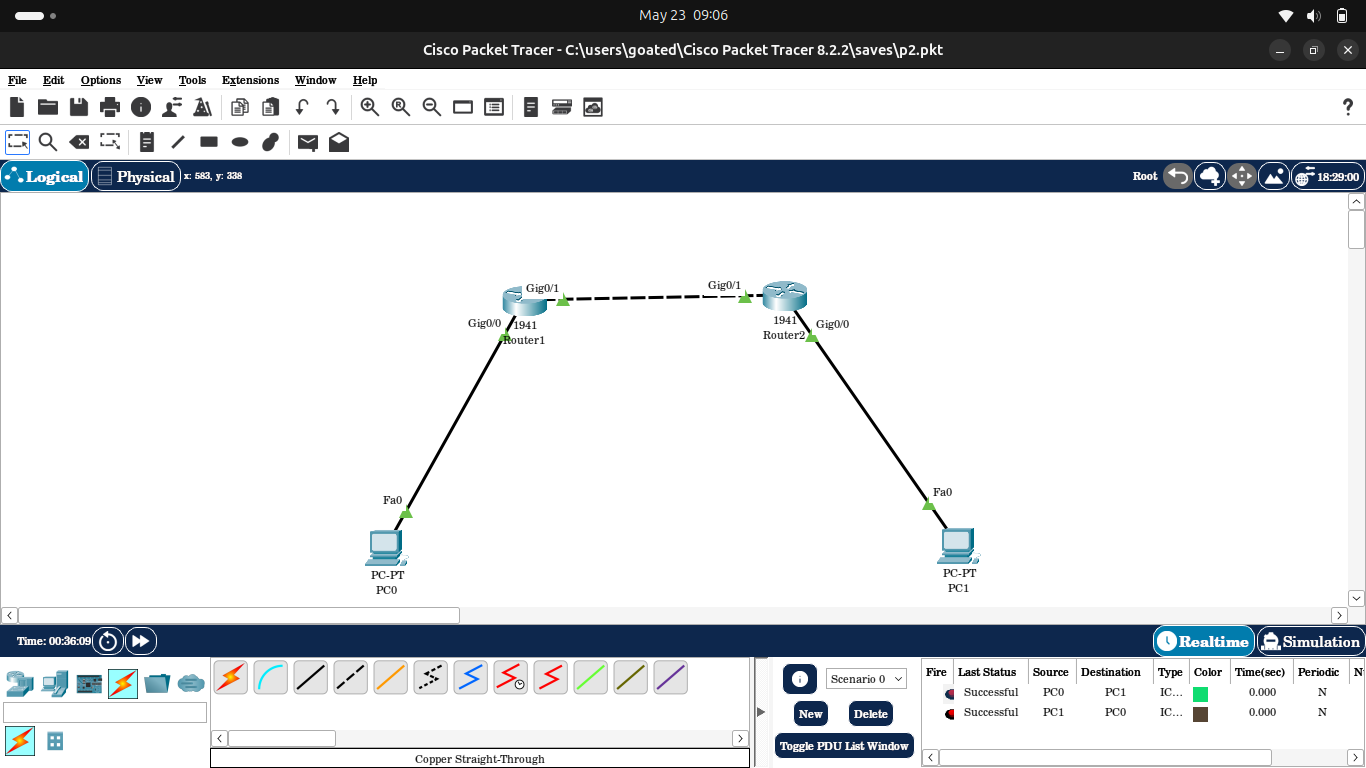
\includegraphics[width=0.5\linewidth]{static.png}
        \caption{Routing Statis IPv6}
        \label{fig:gambar1}
    \end{figure}
    \item  \
    begin{figure}[H]
        \centering
        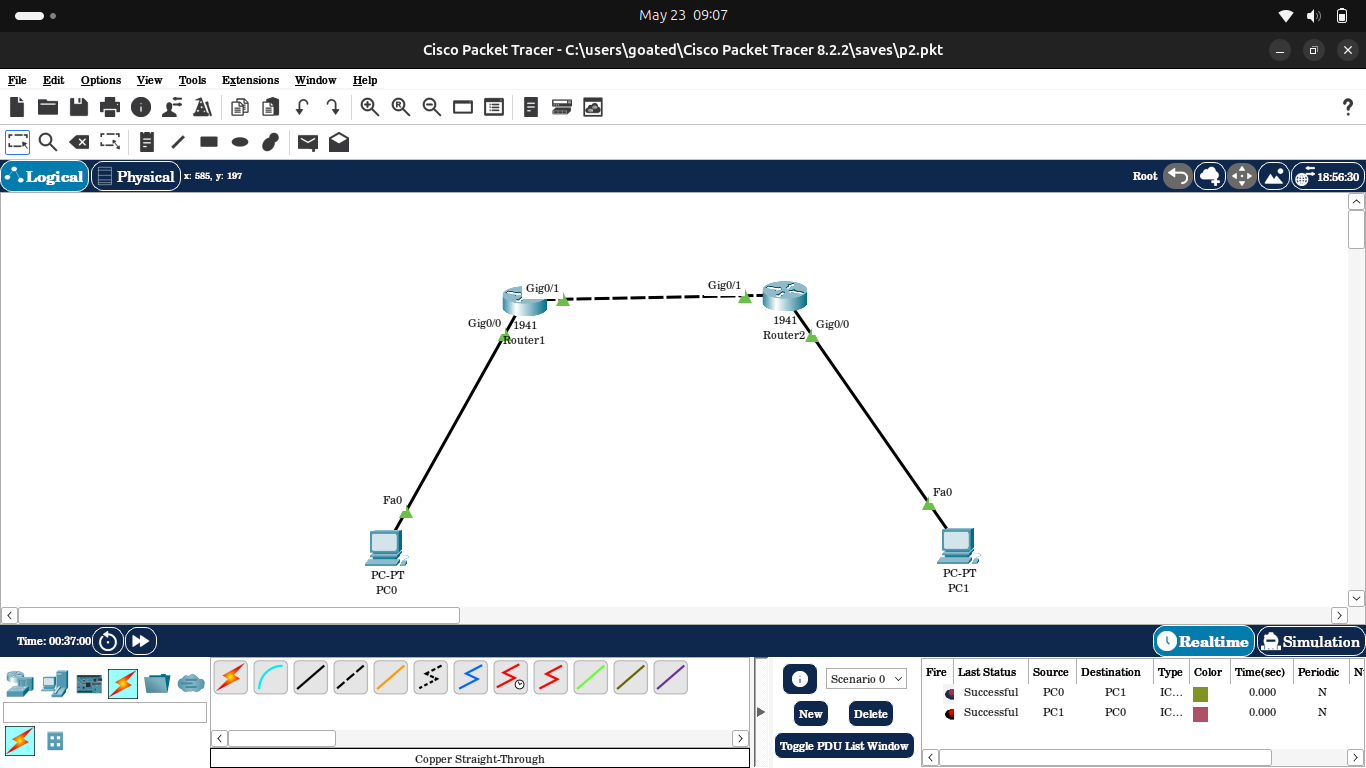
\includegraphics[width=0.5\linewidth]{dynamic.png}
        \caption{Routing Dinamis IPv6}
        \label{fig:gambar1}
    \end{figure}
\end{enumerate}


\section{Kesimpulan}
Dari hasil percobaan yang telah dilakukan, dapat disimpulkan bahwa routing statis IPv6 dan routing dinamis IPv6
dapat dilakukan dengan baik pada jaringan komputer. Routing statis IPv6 dapat digunakan untuk jaringan yang
kecil dan tidak sering mengalami perubahan topologi jaringan, sedangkan routing dinamis IPv6 dapat digunakan untuk
jaringan yang besar dan sering mengalami perubahan topologi jaringan. Routing dinamis IPv6 lebih efisien dan lebih
mudah dikelola dibandingkan dengan routing statis IPv6 karena dapat menyesuaikan diri dengan perubahan topologi
jaringan secara otomatis. Pada routing dinamis IPv6 digunakan OSPF sebagai protokol routing yang dapat menyesuaikan diri
dengan perubahan topologi jaringan secara otomatis.
\section{Lampiran}

\begin{figure}[H]
        \centering
        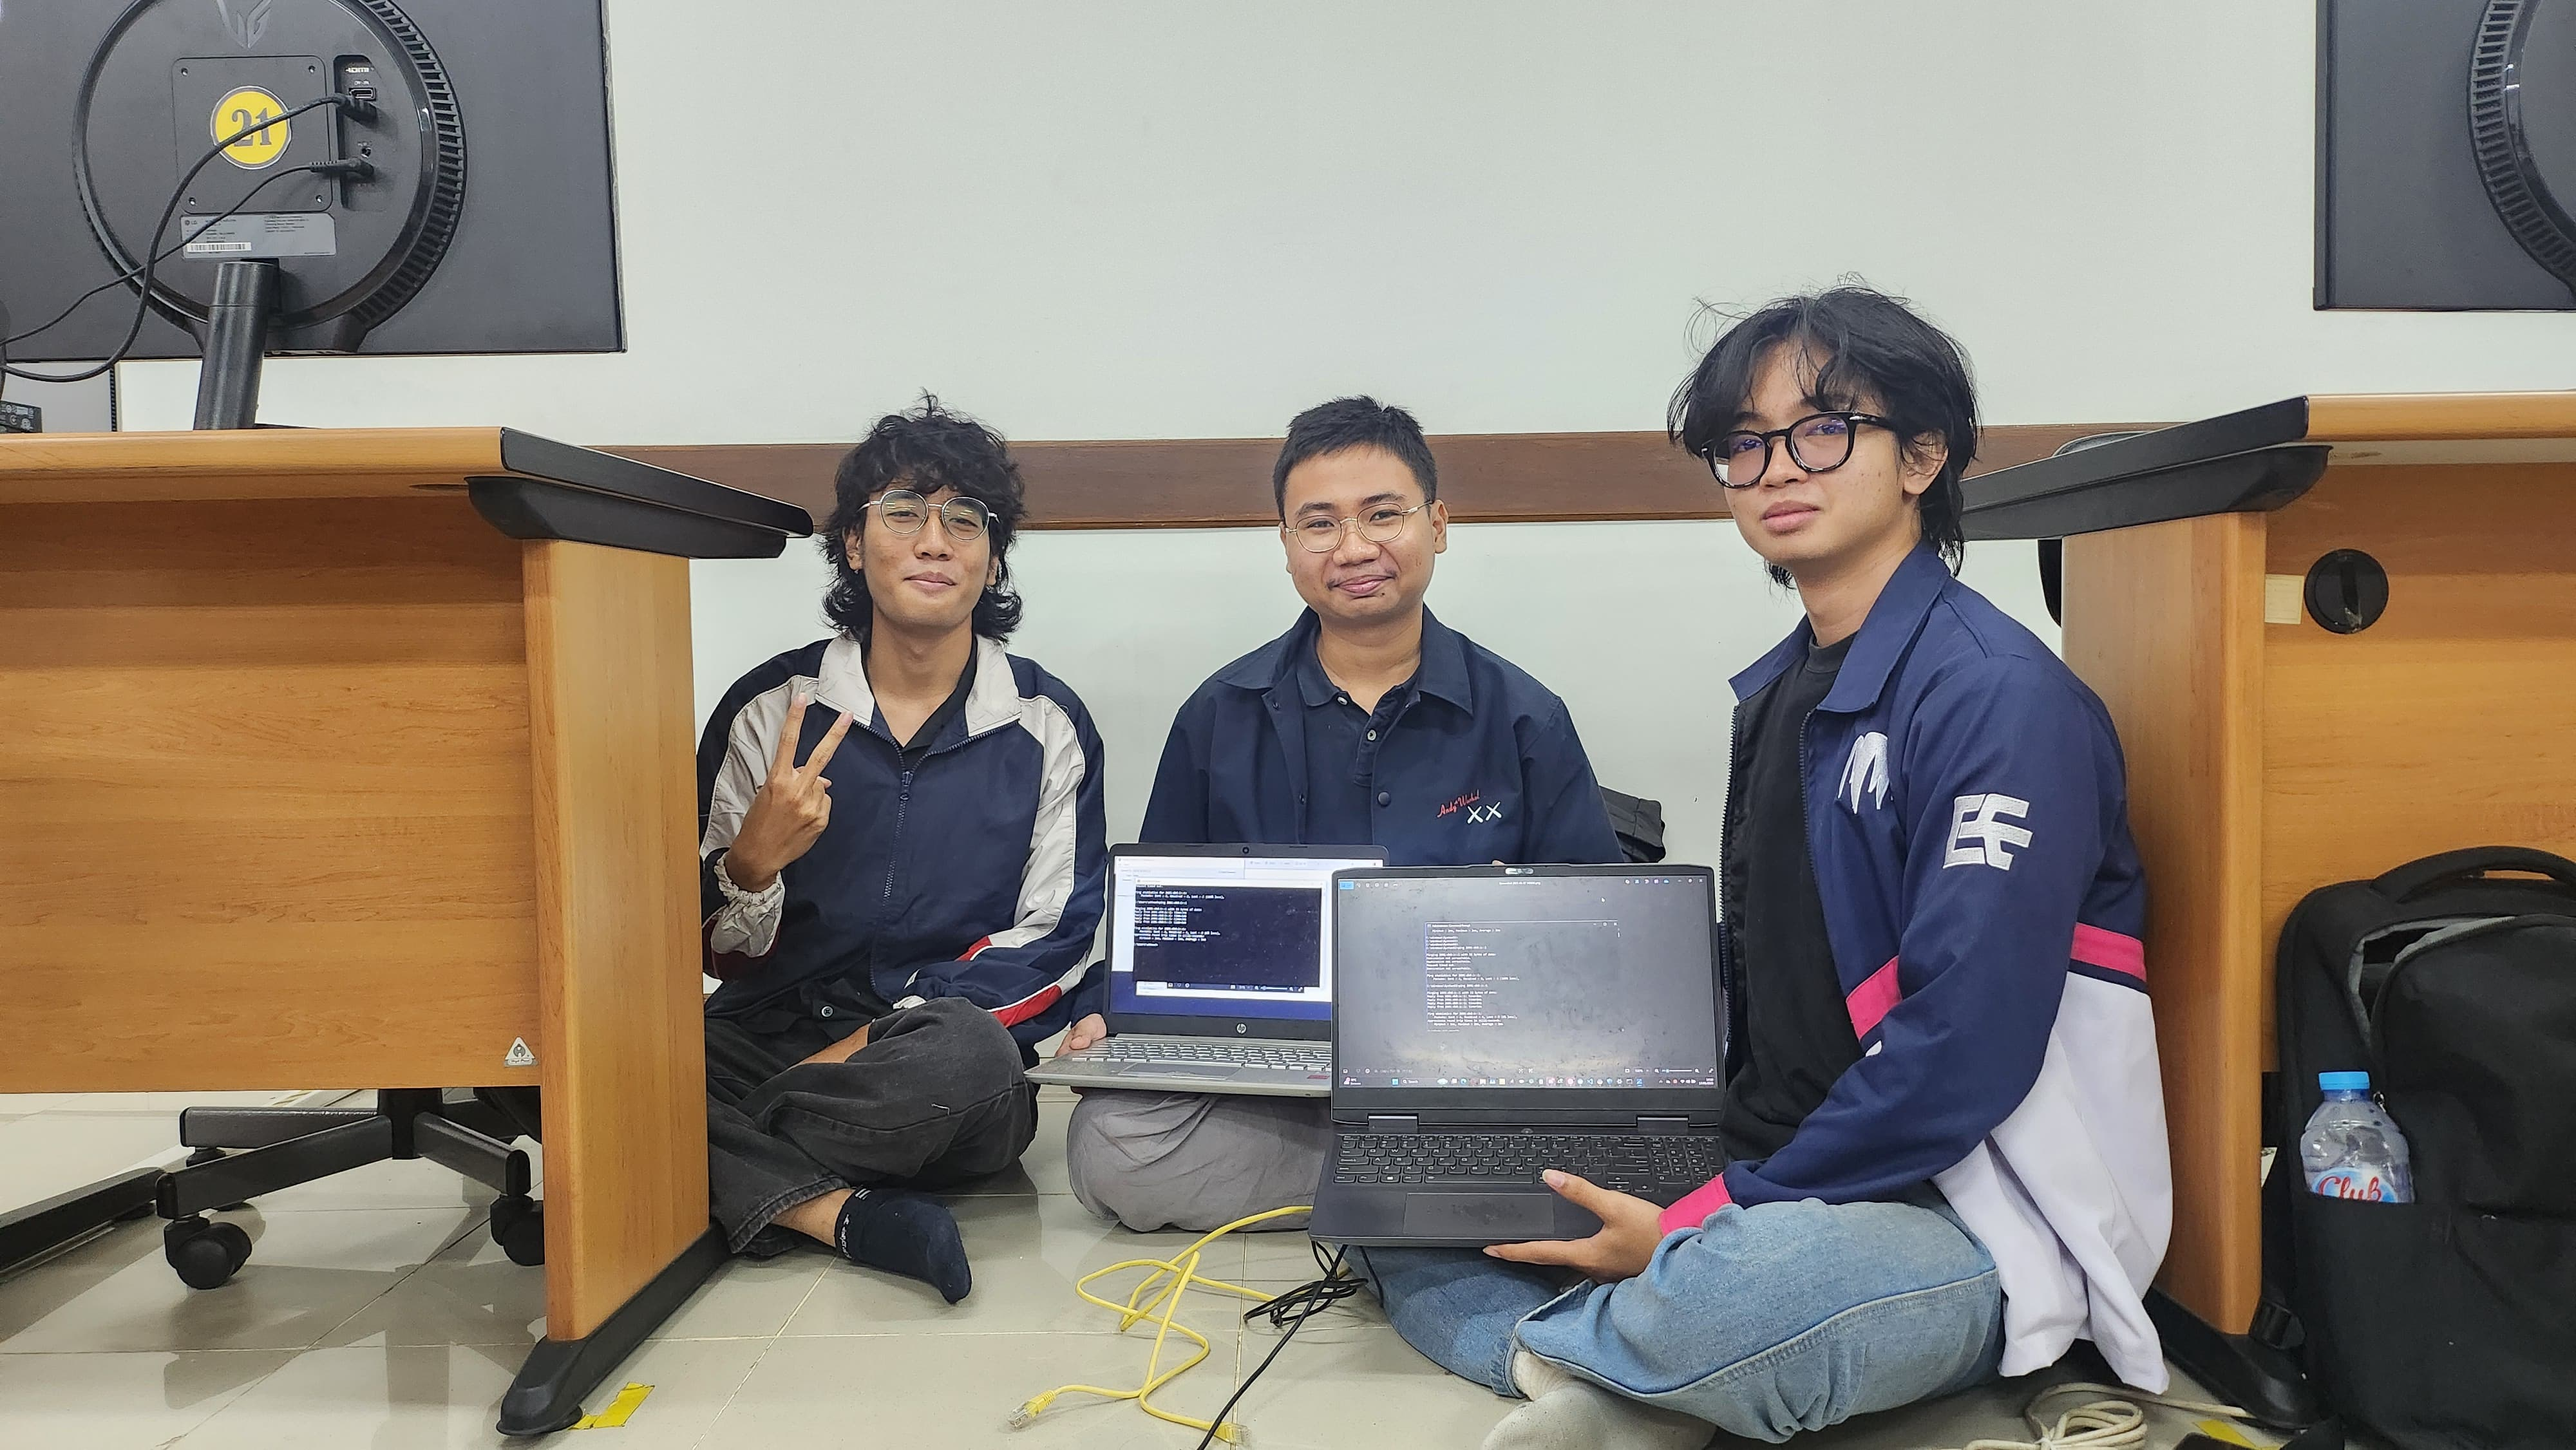
\includegraphics[width=0.5\linewidth]{gambar8.jpeg}
        \caption{Dokumentasi}
        \label{fig:gambar1}
    \end{figure}

    \begin{figure}[H]
        \centering
        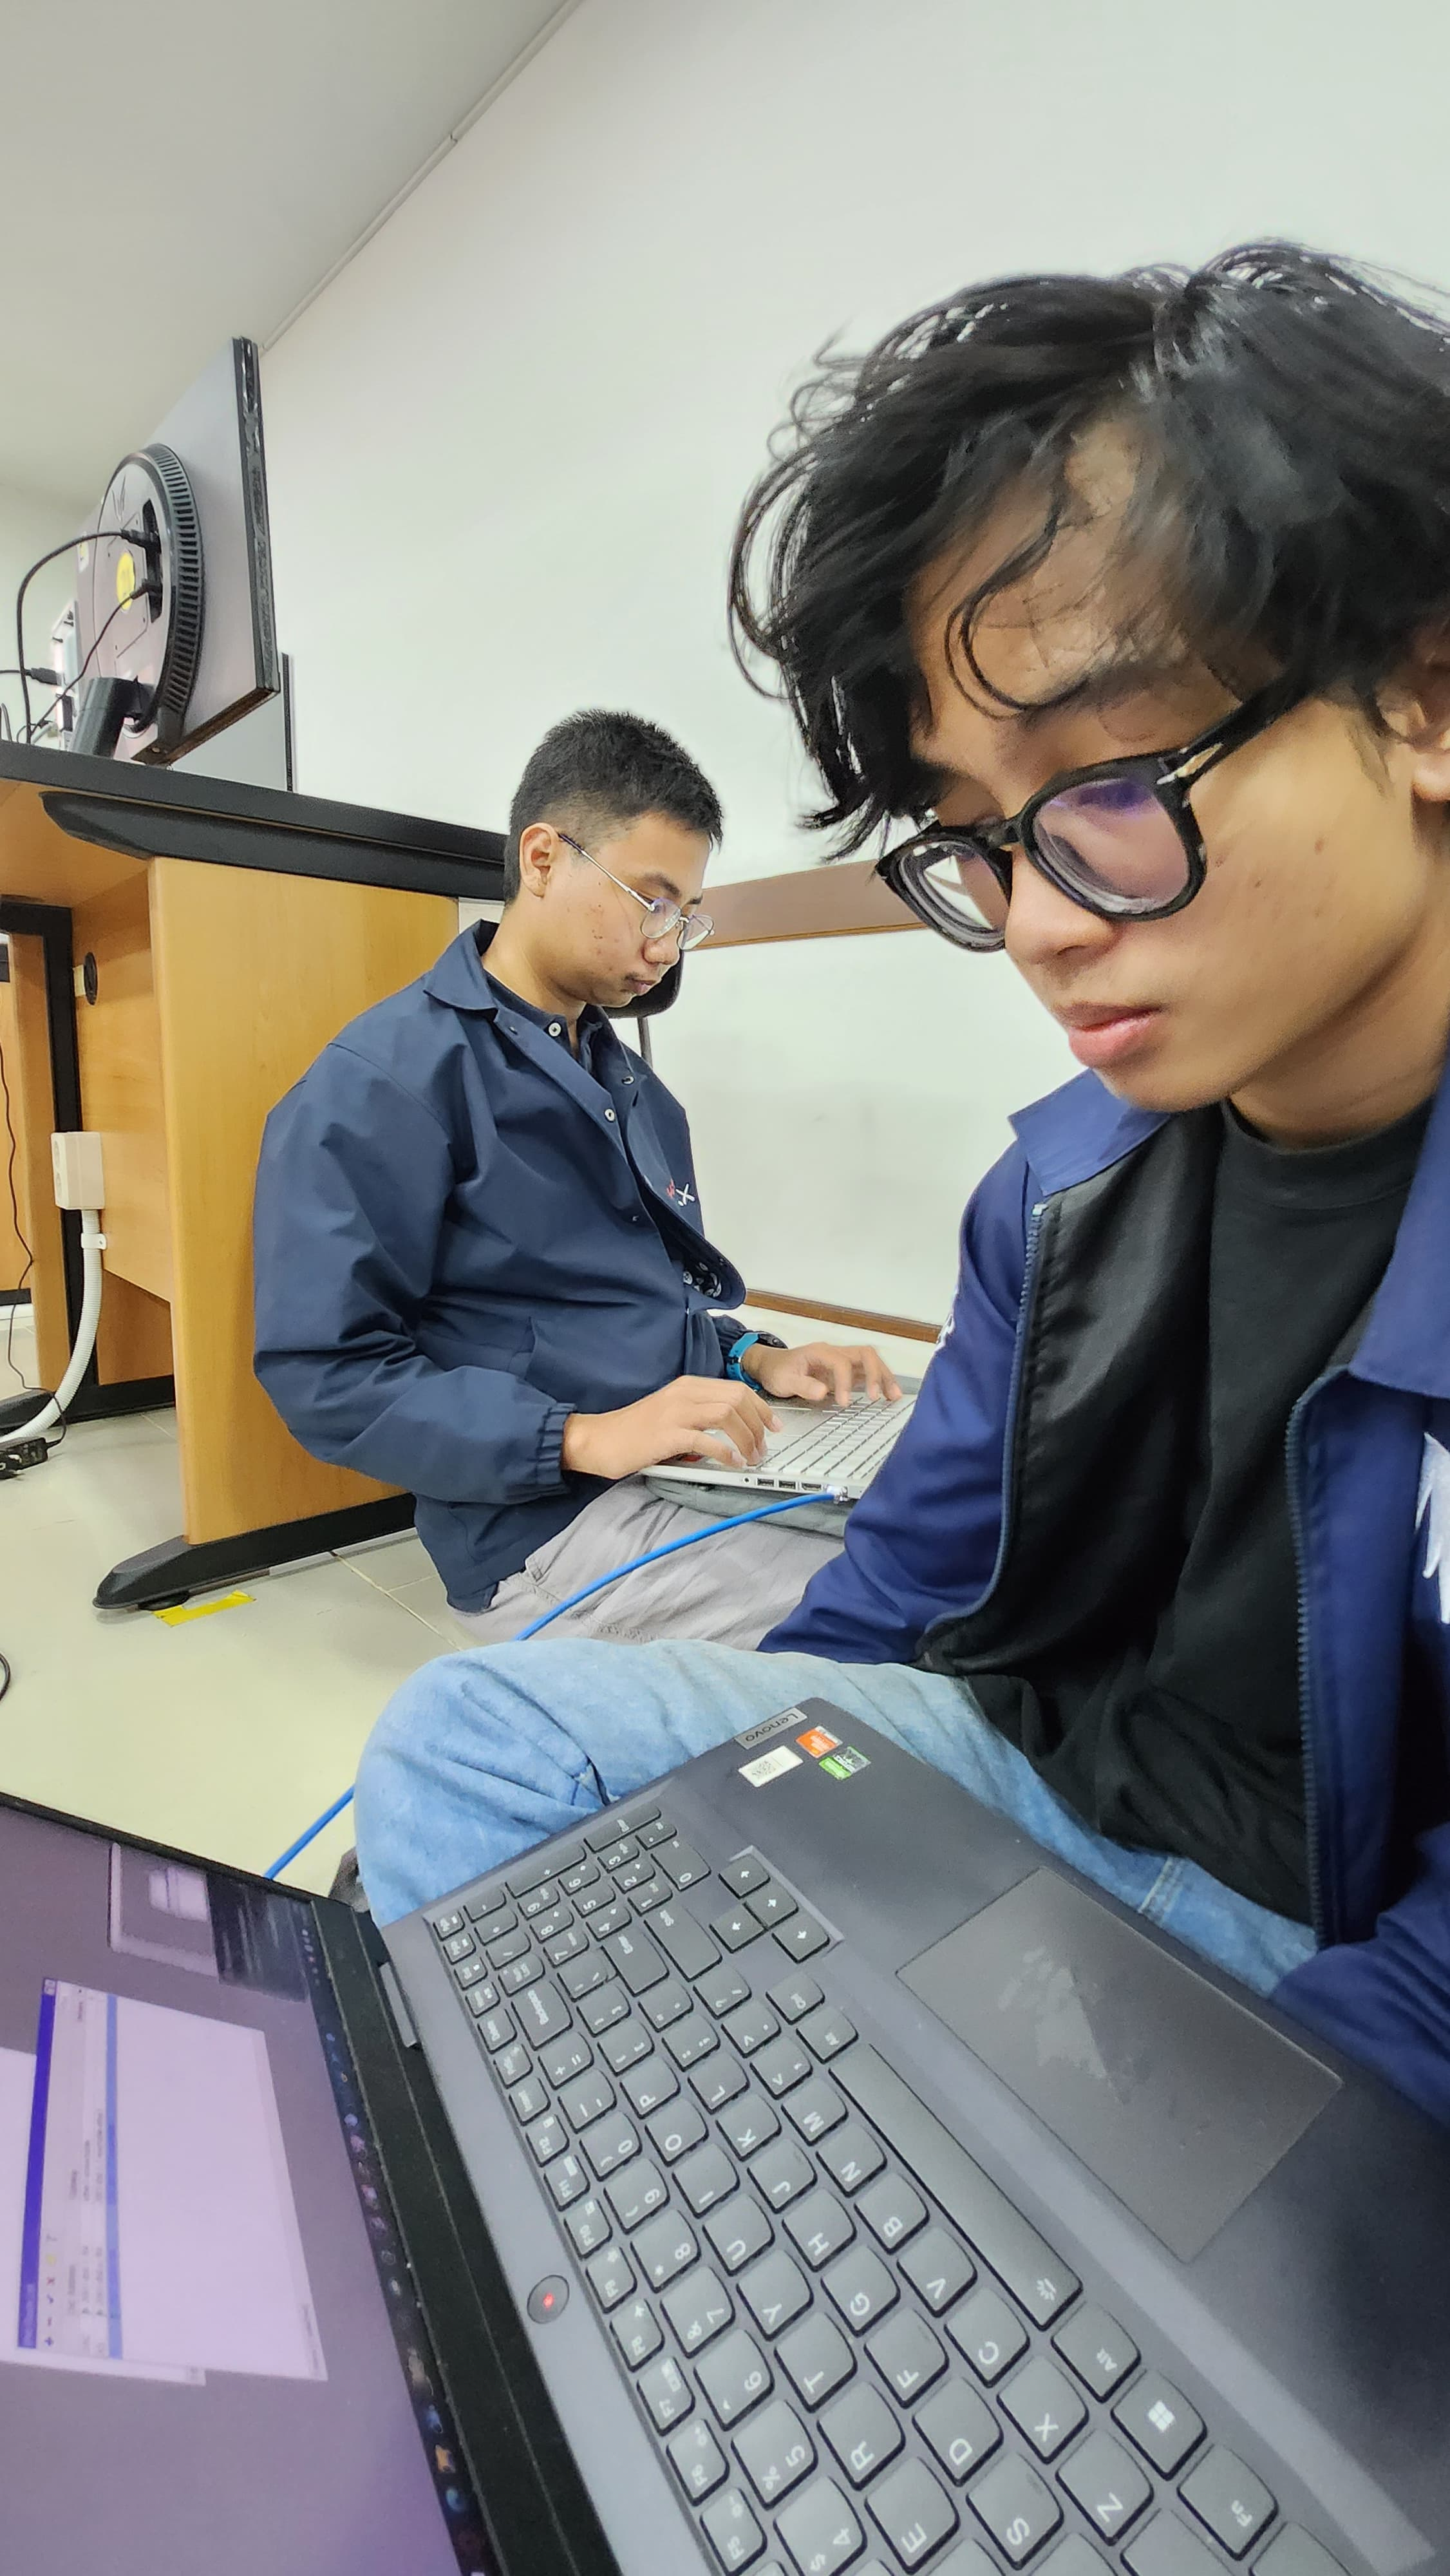
\includegraphics[width=0.5\linewidth]{gambar9.jpeg}
        \caption{Dokumentasi}
        \label{fig:gambar1}
    \end{figure}

    \begin{figure}[H]
        \centering
        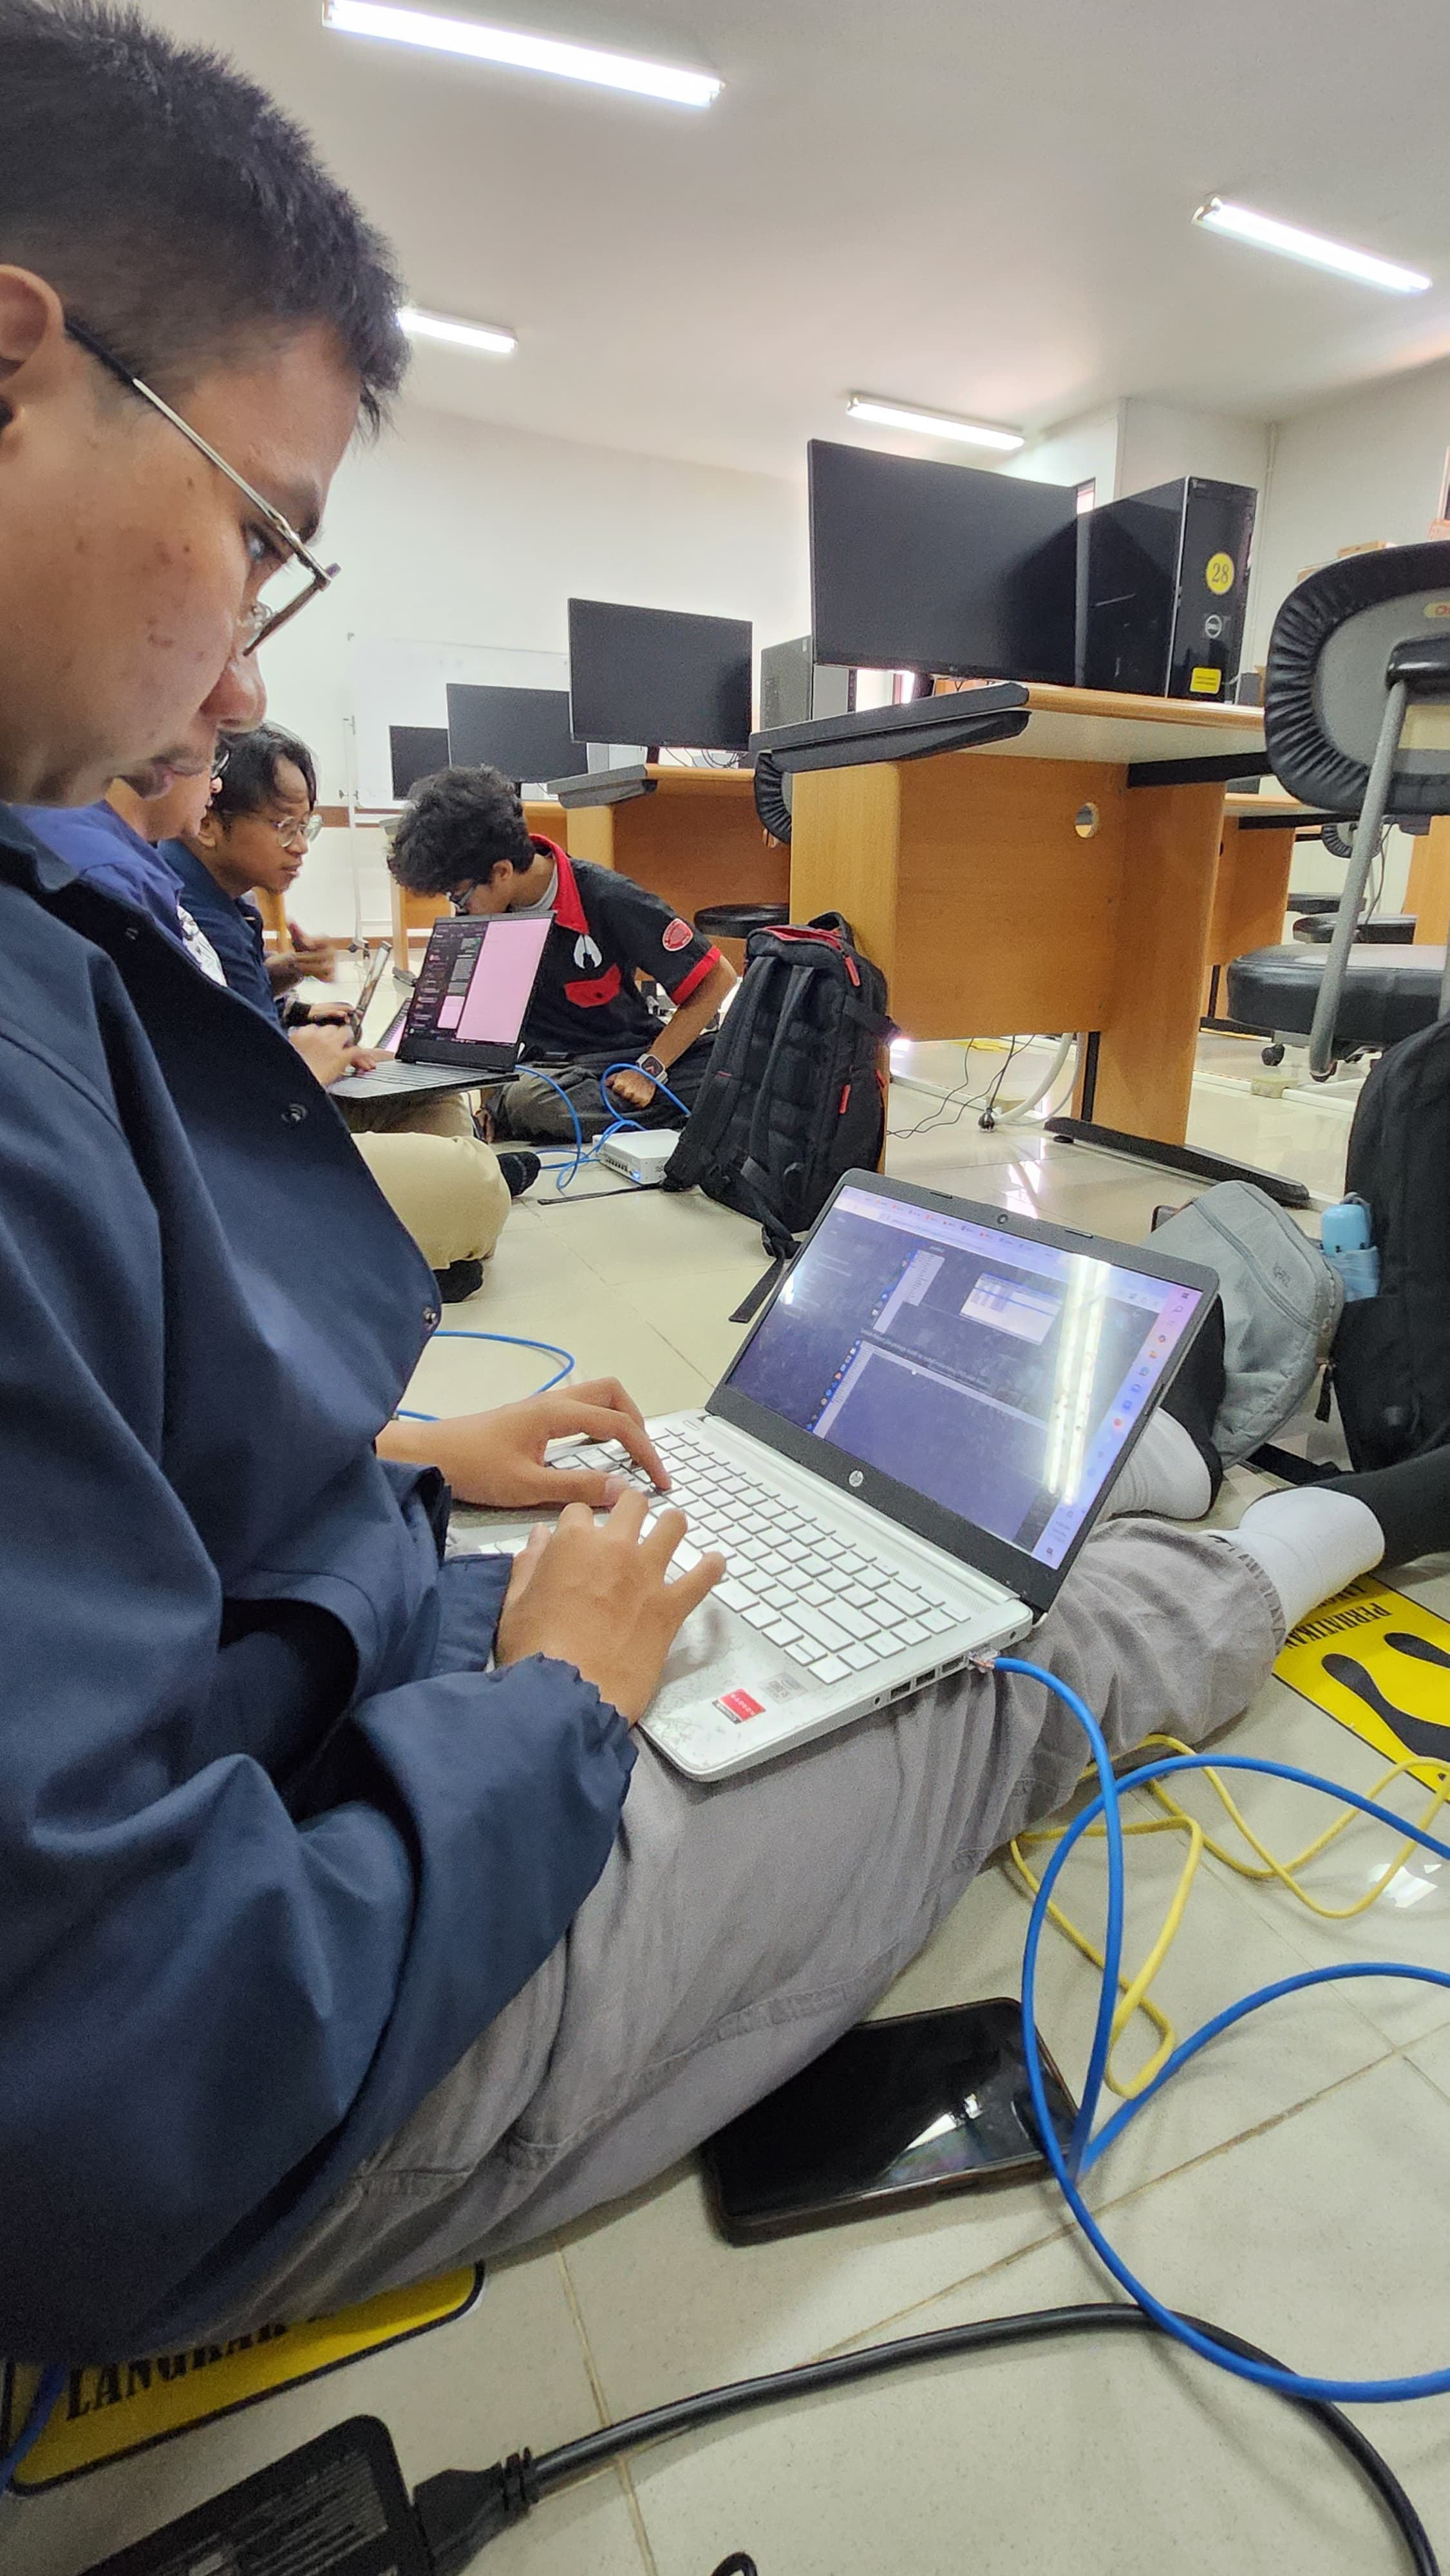
\includegraphics[width=0.5\linewidth]{gambar10.jpeg}
        \caption{Dokumentasi}
        \label{fig:gambar1}
    \end{figure}
    \begin{figure}[H]
        \centering
        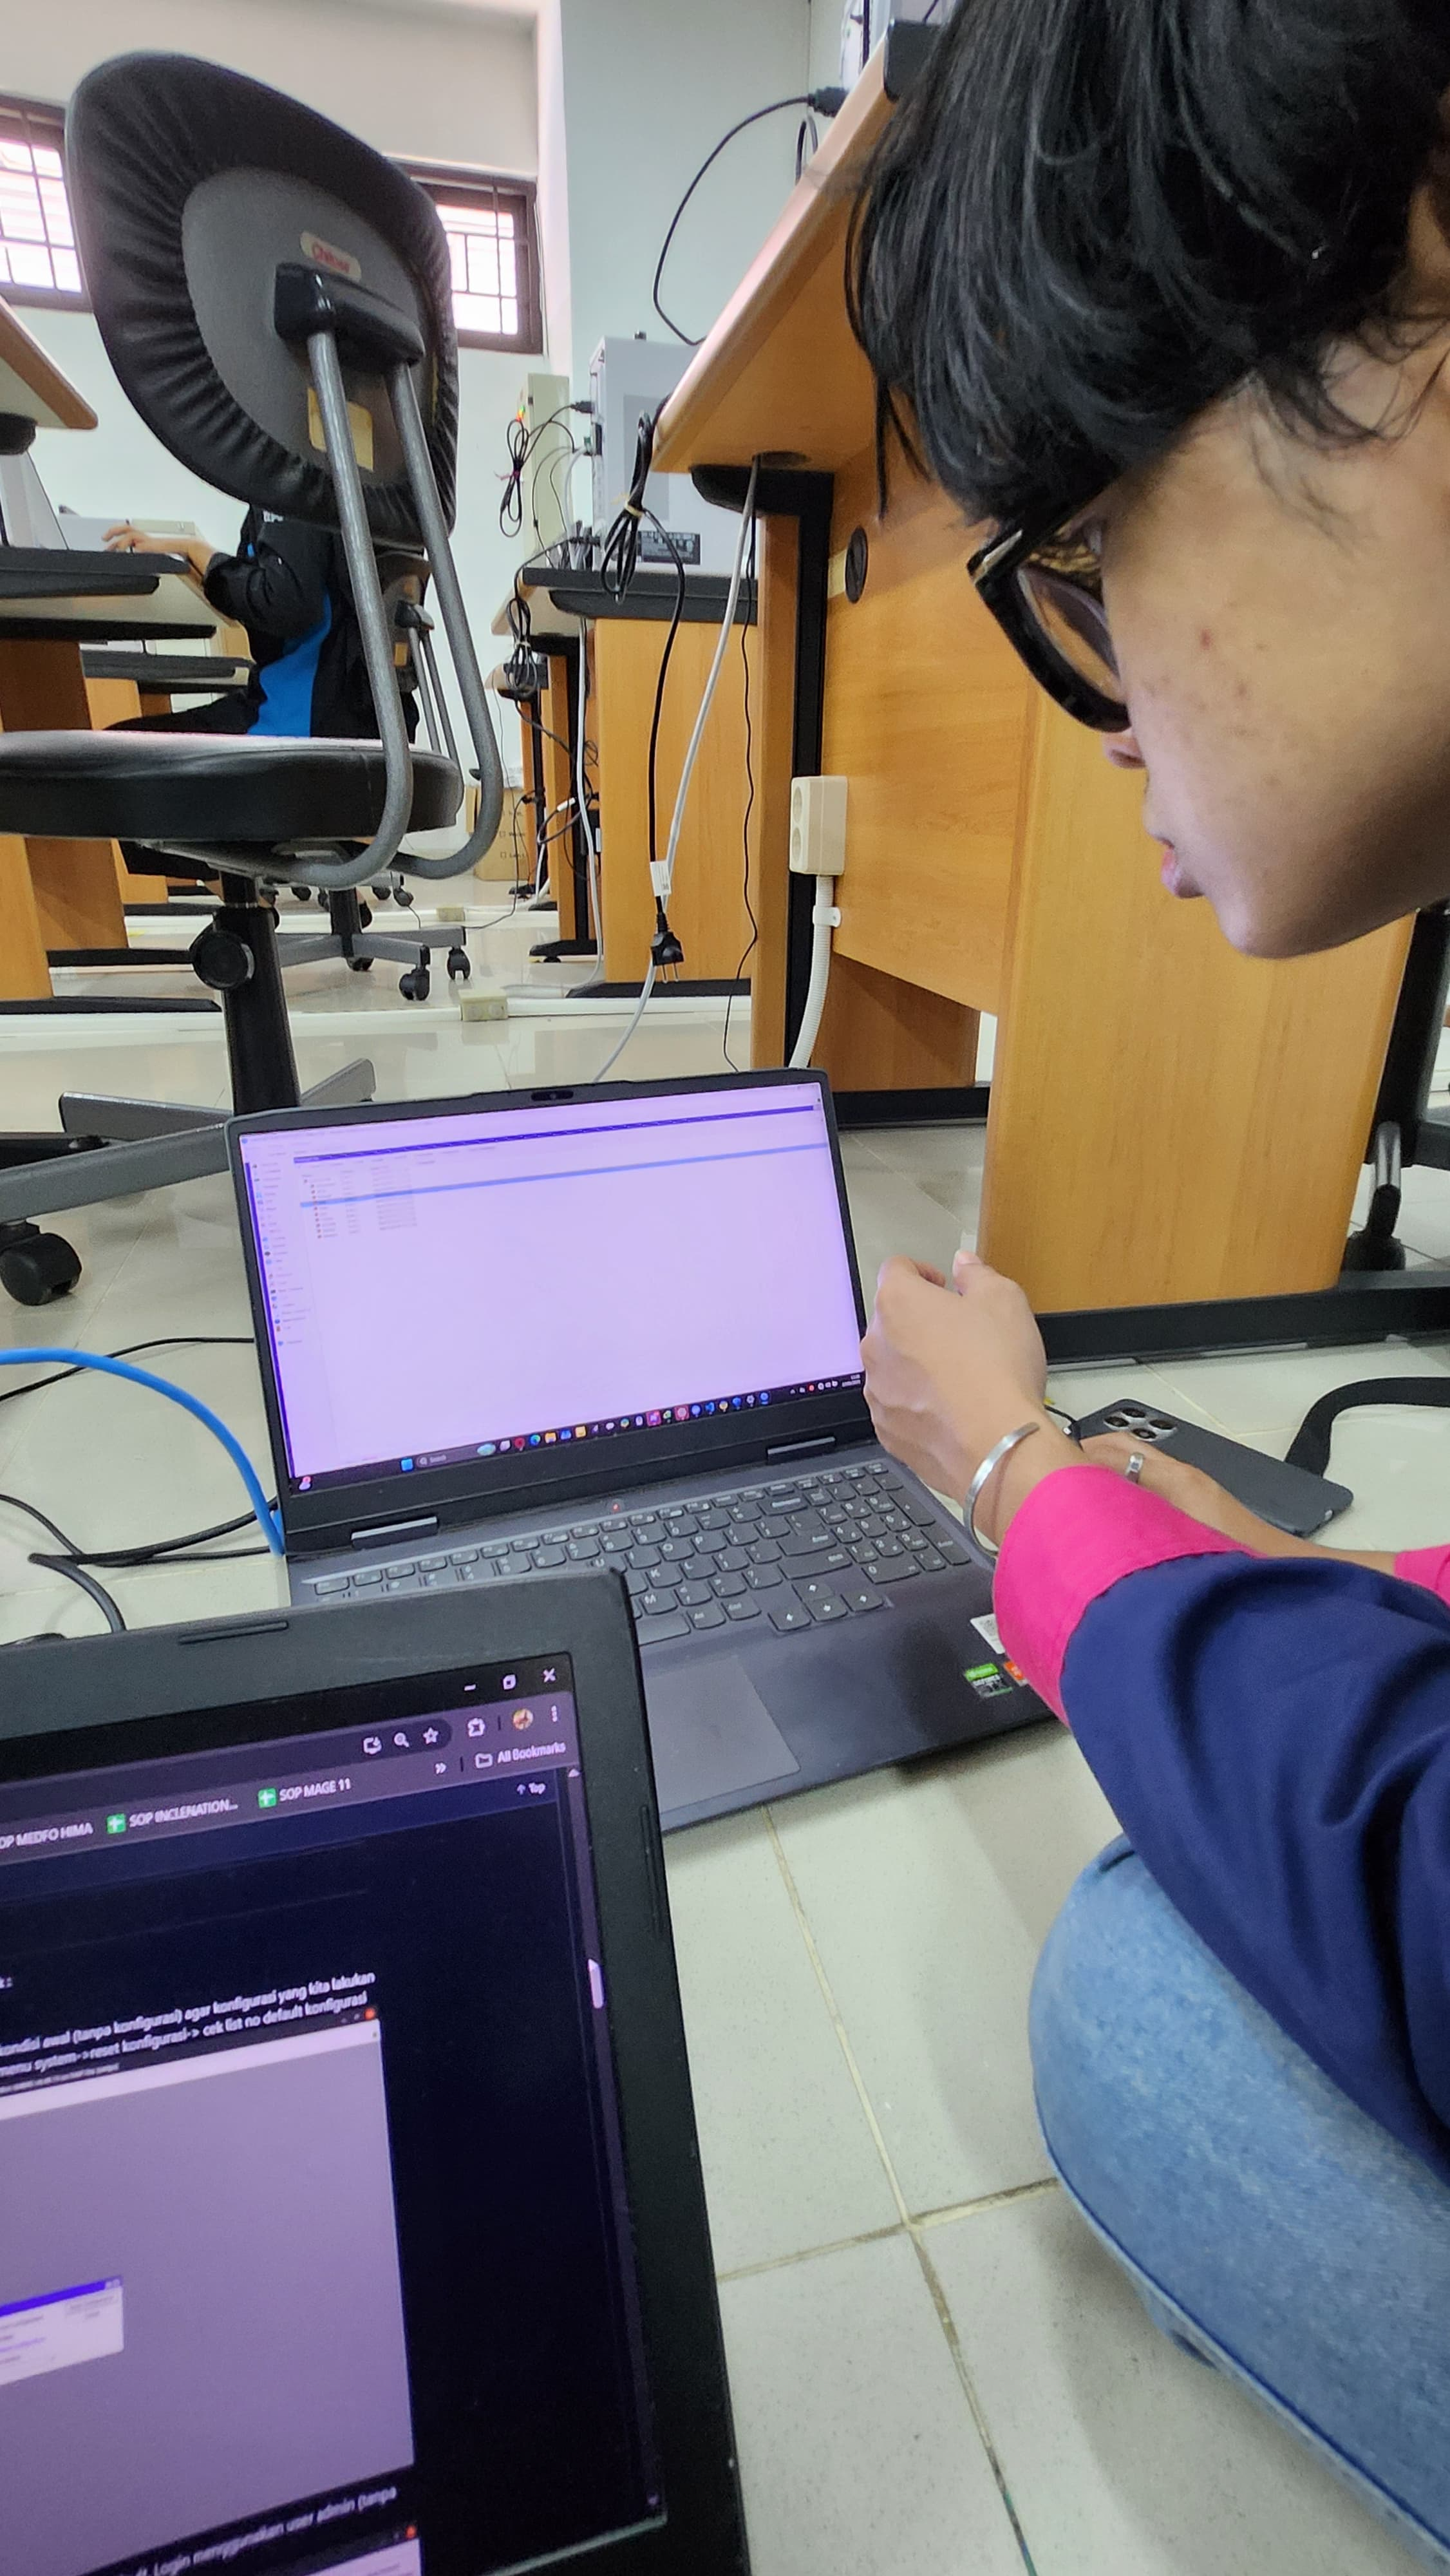
\includegraphics[width=0.5\linewidth]{gambar11.jpeg}
        \caption{Dokumentasi}
        \label{fig:gambar1} 
    \end{figure}
\subsection{Dokumentasi saat praktikum}



